\documentclass{ximera}



\graphicspath{
  {./}
  {ximeraTutorial/}
  {basicPhilosophy/}
}

\newcommand{\mooculus}{\textsf{\textbf{MOOC}\textnormal{\textsf{ULUS}}}}


\usepackage{tkz-euclide}\usepackage{tikz}
\usepackage{tikz-cd}
\usetikzlibrary{arrows}
\tikzset{>=stealth,commutative diagrams/.cd,
  arrow style=tikz,diagrams={>=stealth}} %% cool arrow head
\tikzset{shorten <>/.style={ shorten >=#1, shorten <=#1 } } %% allows shorter vectors

\usetikzlibrary{backgrounds} %% for boxes around graphs
\usetikzlibrary{shapes,positioning}  %% Clouds and stars
\usetikzlibrary{matrix} %% for matrix
\usepgfplotslibrary{polar} %% for polar plots
\usepgfplotslibrary{fillbetween} %% to shade area between curves in TikZ
\usetkzobj{all}
\usepackage[makeroom]{cancel} %% for strike outs
%\usepackage{mathtools} %% for pretty underbrace % Breaks Ximera
%\usepackage{multicol}
\usepackage{pgffor} %% required for integral for loops



%% http://tex.stackexchange.com/questions/66490/drawing-a-tikz-arc-specifying-the-center
%% Draws beach ball
\tikzset{pics/carc/.style args={#1:#2:#3}{code={\draw[pic actions] (#1:#3) arc(#1:#2:#3);}}}



\usepackage{array}
\setlength{\extrarowheight}{+.1cm}
\newdimen\digitwidth
\settowidth\digitwidth{9}
\def\divrule#1#2{
\noalign{\moveright#1\digitwidth
\vbox{\hrule width#2\digitwidth}}}
























%%This is to help with formatting on future title pages.
\newenvironment{sectionOutcomes}{}{}





\title{Functions}

\begin{document}
\begin{abstract}
differentials
\end{abstract}
\maketitle







\section{Differentials}

The  graph of a function $f$ and the graph of $L$, the linear approximation of $f$ at $a$, are shown in the figure below.
Also, two quantities, $dx$ and $df$, and a point $P$ are marked in the figure. Look carefully at the figure when answering the questions below.


\begin{image}
%\begin{marginfigure}[0in]
\begin{tikzpicture}
  \begin{axis}[
            xmin=1, xmax=2, range=0:6,ymax=6,ymin=0,
            axis lines =left, xlabel=$x$, ylabel=$y$,
            every axis y label/.style={at=(current axis.above origin),anchor=south},
            every axis x label/.style={at=(current axis.right of origin),anchor=west},
            ticks=none,
            axis on top,
          ]         
          \addplot [draw=black,dashed,->,>=stealth'] plot coordinates {(1.4,10/6) (1.7,10/6)};
          \addplot [draw=black,dashed,->,>=stealth'] plot coordinates {(1.7,10/6) (1.7,10/6 +.3/.36)};
          \addplot [very thick,penColor, smooth,samples=100,domain=(0:1.833)] {-1/(x-2)};
          \addplot [very thick,penColor2, smooth,samples=100,domain=(0:1.833)] {1/0.6+(1/0.36)*(x-1.4)};
          \addplot[color=penColor,fill=penColor,only marks,mark=*] coordinates{(1.7,1/0.3)};  %% closed hole  
          \addplot[color=penColor3,fill=penColor3,only marks,mark=*] coordinates{(1.7,10/6 +.3/.36)};  %% closed hole  
          \addplot[color=penColor3,fill=penColor3,only marks,mark=*] coordinates{(1.4,10/6)};  %% closed hole            
          \node at (axis cs:1.55,1.67) [below] {$dx$};
          \node at (axis cs:1.7,2.08) [right] {$df$};
          \node at (axis cs:1.15,1.85) [below] {$y=f(x)$};
          \node at (axis cs:1.05,0.55) [right] {$y=L(x)$};
          \node at (axis cs:1.24,2.0) [right] {$(a,f(a))$};
          \node at (axis cs:1.478,3.315) [right] {$(x,f(x))$};
          \node at (axis cs:1.68,2.8) [right] {$P$};
        \end{axis}
\end{tikzpicture}
%\caption{While $dy$ and $\d x$ are both variables, $dy$ depends on $\d x$,
  %and approximates how much a function grows after a change of size
  %$\d x$ from a given point.}
%\label{figure:differentials}
%\end{marginfigure}
\end{image}
\begin{question}
  Select all the correct expressions for the quantity $dx$.
   \begin{hint}
     You can see that $x=a+dx$.
    \end{hint}
    \begin{selectAll}
      \choice{$dx=f(x)-f(a)$}
      \choice{$dx=f(x)-L(x)$}
      \choice[correct]{$dx=x-a$}
      \choice{$dx=L(x)-f(a)$}
      \choice{$dx=L(x)-L(a)$}
    \end{selectAll}
  \end{question}

  
  \begin{question}
  Select all the correct expressions for the quantity $df$.
   \begin{hint}
     You can see that $L(x)=f(a)+df$.
    \end{hint}
      \begin{hint}
    Recall: $L(a)=f(a)$.
    \end{hint}
    \begin{selectAll}
      \choice{$df=f(x)-f(a)$}
      \choice{$df=f(x)-L(x)$}
      \choice{$df=x-a$}
      \choice[correct]{$df=L(x)-f(a)$}
      \choice[correct]{$df=L(x)-L(a)$}    
    \end{selectAll}
  \end{question}











\begin{question}
Based on  the figure and the expression for $L(x)$, select all the correct expressions for $df$.
 \begin{hint}
    Recall: $df=L(x)-f(a)=f(a)+f'(a)(x-a)-f(a)=f'(a)(x-a)=f'(a)dx$.
    \end{hint}
      \begin{selectAll}
      \choice[correct]{ $df=f'(a)(x-a)$}
      \choice[correct]{ $df=f'(a)dx$}
      \choice{$df=f'(x-a)$}
      \choice{$df=f'(x)dx$}
      \choice{$df=f'(x)(x-a)$}
      \end{selectAll}
  \end{question}
  
 So, we can write $df=f'(a)dx$ and call it a \textbf{differential} of $f$ at $a$. Notice that we can define a differential at any number $x$ of the domain of $f$, provided that $f'(x)$ exists.
We will  do that in our next definition.
\begin{definition}
Let $f$ be a differentiable function, let $x$ be a number in the domain of $f$, and let  $dx$ be some quantity, called a \textbf{differential of $x$}.
We define  $df$, a differential of $f$,  at a number $x$ by 
\[
df=f'(x)\cdot dx
\] 

 Geometrically, differentials can be interpreted via the diagram below.
\begin{image}
%\begin{marginfigure}[0in]
\begin{tikzpicture}
  \begin{axis}[
            xmin=1, xmax=2, range=0:6,ymax=6,ymin=0,
            axis lines =left, xlabel=$x$, ylabel=$y$,
            every axis y label/.style={at=(current axis.above origin),anchor=south},
            every axis x label/.style={at=(current axis.right of origin),anchor=west},
            ticks=none,
            axis on top,
          ]         
          \addplot [draw=black,dashed,->,>=stealth'] plot coordinates {(1.4,10/6) (1.7,10/6)};
          \addplot [draw=black,dashed,->,>=stealth'] plot coordinates {(1.7,10/6) (1.7,10/6 +.3/.36)};
          \addplot [very thick,penColor, smooth,samples=100,domain=(0:1.833)] {-1/(x-2)};
          \addplot [very thick,penColor2, smooth,samples=100,domain=(0:1.833)] {1/0.6+(1/0.36)*(x-1.4)};
          \addplot[color=penColor,fill=penColor,only marks,mark=*] coordinates{(1.7,1/0.3)};  %% closed hole  
          \addplot[color=penColor3,fill=penColor3,only marks,mark=*] coordinates{(1.7,10/6 +.3/.36)};  %% closed hole  
          \addplot[color=penColor3,fill=penColor3,only marks,mark=*] coordinates{(1.4,10/6)};  %% closed hole            
          \node at (axis cs:1.55,1.67) [below] {$dx$};
          \node at (axis cs:1.7,2.08) [right] {$df$};
          \node at (axis cs:1.15,1.85) [below] {$f$};
          \node at (axis cs:1.05,0.55) [right] {$L$};
          \node at (axis cs:1.24,2.0) [right] {$(x,f(x))$};
          \node at (axis cs:1.26,3.6) [right] {$(x+dx,f(x+dx))$};
          
        \end{axis}
\end{tikzpicture}
%\caption{While $dy$ and $\d x$ are both variables, $dy$ depends on $\d x$,
  %and approximates how much a function grows after a change of size
  %$\d x$ from a given point.}
%\label{figure:differentials}
%\end{marginfigure}
\end{image}

Note, it is now the case (by definition!) that 
\[
 f'(x)=\frac{df}{dx}.
\]
\end{definition}
We should not be surprised, since the slope of the tangent line in the figure is $f'(x)$,  and this slope is also given by $\frac{df }{dx}$.















Essentially, differentials allow us to solve the problems presented in
the previous examples from a slightly different point of view. Recall,
when $h$ is near but not equal zero,
\[
f'(x) \approx \frac{f(x+h)-f(x)}{h}.
\]
Hence, 
\[
f'(x)h \approx f(x+h)-f(x).
\]
We can replace a quantity $h$ with a quantity $dx$ to write
\begin{align*}
f'(x)\cdot dx &\approx f(x+dx)-f(x)\\
df &\approx f(x+dx)-f(x).
\end{align*}
Adding $f(x)$ to both sides we see
\[
f(x) + df\approx f(x+dx)
\]
or, equivalently
\[
f(x+dx)\approx f(x) + df .
\]
There
are contexts where the language of differentials is common. Here is
the basic strategy:
\begin{image}
  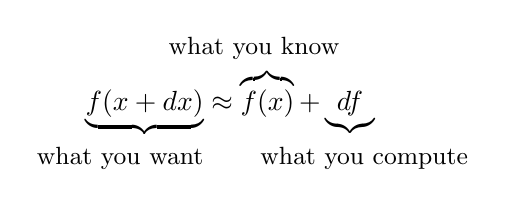
\begin{tikzpicture}
    \node at (0,0) {
      $\underbrace{f(x + dx)} \approx  \overbrace{f(x)} + \underbrace{df}$
    };
    \node at (-1.4,-.7) {\small{what you want}};
    \node at (.3,.7) {\small{what you know}};
    \node at (1.7,-.7) {\small{what you compute}};
  \end{tikzpicture}
\end{image}

We will repeat our previous examples using differentials.

\begin{example}
Use differentials to approximate $\sqrt[3]{50}$.
\begin{explanation}
  Set $f(x) = \sqrt[3]{x}$. We want to know $\sqrt[3]{50}$.  Since
  $4^3 = 64$, we set $x=64$.  Setting $dx=50-64=-14$, we have
  \begin{align*}
  \sqrt[3]{50} = f(x + dx) &\approx  f(x) + df\\
  &\approx \sqrt[3]{64} + df.
  \end{align*}
  Here we see a plot of $y=\sqrt[3]{x}$ with the differentials above
  marked:
  \begin{image}
    \begin{tikzpicture}
      \begin{axis}[
          xmin=40,xmax=70,ymin=3,ymax=4.5,
          axis lines=center,
          xlabel=$x$, ylabel=$y$,
          every axis y label/.style={at=(current axis.above origin),anchor=south},
          every axis x label/.style={at=(current axis.right of origin),anchor=west},
        ]        
        \addplot [very thick, penColor, samples=150,smooth,domain=(0:100)] {x^(1/3))};
        %\addplot [very thick, penColor2, domain=(50:64)] {x/48+8/3};
        %\addplot [textColor,dashed] plot coordinates {(64,0) (64,4)};
        \addplot [draw=black,dashed,->,>=stealth'] plot coordinates {(50,4) (50,3.71)};
        \addplot [draw=black,dashed,->,>=stealth'] plot coordinates {(64,4) (50, 4)};
        \addplot [very thick, penColor2, domain=(0:100)] {x/48+8/3};
        \node [above] at (axis cs:57,4) {$dx$};
        \node [left] at (axis cs:50,3.86) {$df$};
        \node [below,penColor3] at (axis cs:64,4) {$(64,4)$};
        \addplot[color=penColor3,fill=penColor3,only marks,mark=*] coordinates{(64,4)};  %% closed hole    
        \node at (axis cs:45,3.5) [penColor] {$f$};
        \node at (axis cs:45,3.67) [penColor2] {$L$};        
      \end{axis}
    \end{tikzpicture}
    %\caption{A plot of $f(x) = \sqrt[3]{x}$  along with the differentials $\d x$ and $dy$.}
    \label{figure:diff sqrt3x}
  \end{image}
  Now we must compute $df$:
  \begin{align*}
    df &= f'(x) \cdot dx\\
    &= \answer[given]{\frac{1}{3x^{2/3}}} \cdot dx\\
    &= \frac{1}{3\cdot64^{2/3}} \cdot(\answer[given]{-14})\\
    &= \frac{1}{3\cdot64^{2/3}} \cdot(-14)\\
    &= \frac{-7}{24}
  \end{align*}
  Hence $f(50) \approx f(64) + \frac{-7}{24} \approx 3.71$.
\end{explanation}
\end{example}









\begin{example}
Use differentials to approximate $\sin(0.3)$.
\begin{explanation}
Set $y = \sin(x)$. We want to know $\sin(0.3)$. Since $\sin(0) = 0$,
we will set $x = 0$ and $dx=0.3$. Write with me
\begin{align*}
  \sin(0.3) = \sin(x + dx) &\approx  \sin(x) + dy\\
  &\approx 0 + dy.
  \end{align*}
  Here we see a plot of $y=\sin(x)$ with the differentials above
  marked:
  \begin{image}
%\begin{marginfigure}
\begin{tikzpicture}
  \begin{axis}[
            xmin=-1,xmax=1,ymin=-1,ymax=1,
            axis lines=center,
            xtick={-1.57, 0, 1.57},
            xticklabels={$-\pi/2$, $0$, $\pi/2$},
            ytick={-1,1},
            %ticks=none,
            %width=3in,
            %height=2in,
            unit vector ratio*=1 1 1,
            xlabel=$x$, ylabel=$y$,
            every axis y label/.style={at=(current axis.above origin),anchor=south},
            every axis x label/.style={at=(current axis.right of origin),anchor=west},
          ]        
          \addplot [very thick, penColor, samples=100,smooth, domain=(-1.6:1.6)] {sin(deg(x))};
          %\addplot [penColor2,very thick] plot coordinates {(0,0) (.3,0)};
          %\addplot [penColor2,very thick] plot coordinates {(.3,0) (.3,.3)};
          \addplot [draw=black,dashed,->,>=stealth'] plot coordinates {(0,0) (.3, 0)};
          \addplot [draw=black,dashed,->,>=stealth'] plot coordinates {(.3,0) (.3, .3)};
          \addplot [thick, penColor2,smooth] {x};
          \node at (axis cs:0.86,0.67) [penColor] {$f$};
          \node at (axis cs:0.86,0.955) [penColor2] {$L$};
          \node [below] at (axis cs:.15,.0) {$dx$};
          \node [right] at (axis cs:.3,.15) {$dy$};
          \node [above left, color=penColor3] at (axis cs:0,0) {$(0,0)$};
          \addplot[color=penColor3,fill=penColor3,only marks,mark=*] coordinates{(0,0)};  %% closed hole          
        \end{axis}
\end{tikzpicture}
%\caption{A plot of $f(x) = \sin(x)$ along with the differentials $\d x$ and $dy$.}
\label{figure:diff sin}
%\end{marginfigure}
\end{image}
Now we must compute $dy$:
\begin{align*}
  dy &= \left(\frac{d}{dx} \sin(x)\right) \cdot dx\\
  &=\answer[given]{\cos(0)} \cdot dx\\
  &= 1 \cdot (\answer[given]{0.3})\\
  &= 0.3
\end{align*}
Hence $\sin(0.3) \approx \sin(0) + 0.3 \approx 0.3$.
\end{explanation}
\end{example}













The upshot is that linear approximations and differentials are simply
two slightly different ways of doing the exact same thing.






\end{document}
